%!TEX root = ../template.tex
%%%%%%%%%%%%%%%%%%%%%%%%%%%%%%%%%%%%%%%%%%%%%%%%%%%%%%%%%%%%%%%%%%%%
%% chapter3.tex
%% NOVA thesis document file
%%
%% Chapter with a short laext tutorial and examples
%%%%%%%%%%%%%%%%%%%%%%%%%%%%%%%%%%%%%%%%%%%%%%%%%%%%%%%%%%%%%%%%%%%%
\chapter{Requirements and Analysis}
\label{cha:requirements_and_analysis}

As previously stated, the main goal of this dissertation is the development of an efficient and effective visual interface for query formulation. The design process phase is the first phase of the solution development, where all the existing relevant problems are combined and took into account in order to draft some possible solutions based on the problem requirements. For this to happen, this chapter describes the processes used to structure the problems of the current visual interface. Furthermore, target users of the system are presented and categorized, accordingly with their background, expectations, and necessities.

\section{Problem Definition}
\label{sec:problem_definition}

The problem definition not only was the starting point of the design process but it also represented the source of the planed solution. As the actual visual interface has not been having the expected acceptability due to its interaction problems, these are problems that have an impactful role in the solution building process. In that way, multiple approaches were used to collect interaction problems, understanding for each of them what are the tasks involved, and the most harmed set of users.

The following sections describe the implemented strategies to define the problem as completely as possible. The result of those analyses was combined in a table that characterizes each problem identified of the existing interface. This table is presented in \nameref{app:taxonomy_of_problems_existing_interface} and describes all the problems identified. For each problem, it is detailed the interface components involved and the Nielsen Heuristics \cite{nielsen_heuristics} affected. Moreover, the issues are classified according to the artifact and task attributes of a Framework adapted from Usability-ODC Framework \cite{in_process_usability_problem_classification_analysis_improvement}, as well as it contains information regarding OutSystems Community\cite{outsystems_community} posts and likes related to each problem.

Hereinafter, the approaches and strategies used to collect and organize data regarding the existing problems of the interface will be presented. As usability issues depend on interaction with users, it was important to analyze the problems holistically, considering, in each problem, the impact caused on each type of user.

\subsection{Analysis}
\label{subsec:analysis}

The analysis of the query formulation interface through self-exploration was the first method used to comprehend the existing problems. The process started with the visualization of two OutSystems tutorials \cite{outsystems_tutorial_aggregates_101, outsystems_tutorial_advanced_aggregates} about visual data querying. The tutorials included some hands-on exploration that provided an initial contextualization of the visual query builder and its functionalities. After that, other scenarios of query formulation were explored to comprehend the system barriers and difficulties.

As pointed out in \ref{sec:problem_description}, the lack of some advanced functionalities were observed during that exploration process. Nevertheless, other problems, which have a negative effect on user experience and task efficiency and effectiveness, were also identified.

First of all, it was detected that some functionalities were hidden, damaging the learnability of the system, not fulfilling the "Recognition rather than recall" principle of the Nielsen Heuristics \cite{nielsen_heuristics}. Notwithstanding that the learnability issue mainly affects the novice users, there are peculiarities of this system and its environment that aggravate this problem. Since SQL formulation is an alternative approach to build queries, if SQL users do not find the intended functionalities in the visual query builder due to its hiddenness, they could use SQL to perform their tasks, avoiding the use of the visual system.

The hidden functionalities are not only advanced features of query formulation. For instance, there is no visible option in the existing interface to add an aggregation function, such as Group By, SUM, MIN, MAX, AVERAGE, or COUNT. These functions are accessible for an exclusive interaction path which requires a right-click on the column header of the attribute where the user intends to apply the aggregation function. Figure \ref{fig:rightClickGroupBy} illustrates an example of the application of an aggregation function. Other options are not always hidden but are not prepared to keep visible due to interface components modification. For example, despite the option to add calculated attributes is visible (after all columns of the query result table), if the query result has several columns it is necessary to scroll horizontally until the end to find that option.

\begin{figure}[htbp]
	\centering
	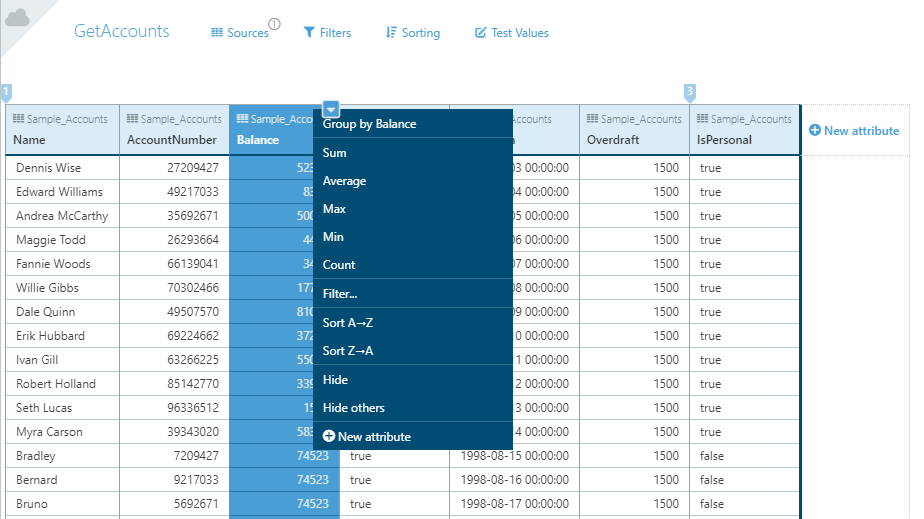
\includegraphics[height=2.5in]{right-click-group-by}
	\caption{Hidden option to add an aggregation function, since it is enclosed in a right-click on the query result table column header.}
	\label{fig:rightClickGroupBy}
\end{figure}

Furthermore, the interface has not revealed to be flexible, efficient, and effective for professional users' purposes. Obstacles have been identified as preventing users from accelerating their query formulation process and causing increases in the queries' error rates. It is presented some examples of these aspects which were identified through the interface's analysis, hindering query formulation and query comprehension, and reducing the most valued proposition of the data querying visual approach:
%TODO: Reference to the most valued proposition.

\begin{itemize}
    \item Search engines: there is no option to efficiently search for an attribute neither to look for some data in the query result or to apply some aggregation function (as illustrated in Figure \ref{fig:rightClickGroupBy}). Moreover, there is no general search in all queries, which could be useful when users need to find if some entity or variable is present in the query.
    \item Hidden columns: in the existing interface, primary and foreign keys are automatically hidden in the query result table since are considered as not relevant data for the query output. That strategy has been implemented since the first release of the interface to provide the most clear output for users with lack of technical background, assuming that they could not understand the meaning of those attributes. Since those attributes may contain relevant information, it is possible to unhide them. However, it must be highlighted that there is no efficient way to expand all hidden columns at once, difficulting significantly the comprehension and formulation of all queries who do not have a reduced number of entities and attributes. Figure \ref{fig:hiddenAttributes} illustrates how the hidden attributes are presented in the interface.
    \item Filter edition: the adaptability of existing query filters is possible using the expression editor modal, as demonstrated in Figure \ref{fig:aggregateFilterModal}. This modal is useful because it provides some guidance in the expression formulation. Users, can select the intended language expressions or the entities, attributes, or variables that need without having to recall those names. However, if users do not need that assistance, the interaction strategy implemented could led to time and visual context wastefulness every time that a modal is opened. It should be noted that the modal is definitely a good feature but it should not be the unique way to edit filters since it can increase the time spent to built queries unnecessarily. Moreover, there is no way to copy and past filter or to read effectively the content since there is no color highlighting in filters expressions.
    \item Accelerators feedback: this visual query interface has multiple accelerators that turn the query building process faster. Nevertheless, sometimes the automatic mechanisms are silent and users may not comprehend they were applied. For example, when two entities are added and are related, the system automatically joins those entities. However, there is no highlight or other visual interaction mechanism that provides feedback to the user and shows him what action were applied in the aggregation output.
    \item Inconsistency problems: some functionalities were accessible through a determined context and option but other alternative options do not have the same behavior. For instance, in some use cases it is not possible to add a new entity to the query using drag and drop but if the user click in another add button the entity is added.
    \item Multiple actions at once: sometimes it could be useful to do several actions at once in order to reduce the time spent to build the query. For instance, it should be possible to add multiple entities at once instead of adding one at a time; 
\end{itemize}

As mentioned, the list of all problems identified is presented in \nameref{app:taxonomy_of_problems_existing_interface}.

In a nutshell, the first analysis and exploration of the interface lead to conclude that the interface is useful for users without technical background and has implemented good strategies that could optimize the query formulation process even more than \gls{SQL} if those strategies would be reconsidered and redesigned. Moreover, it was concluded that it is necessary to provide search engines and other accelerators to enhance the efficiency value proposition of the system. The value of the system increases if users could build queries in that system as fast as \gls{SQL} or even more.

\begin{figure}[htbp]
	\centering
	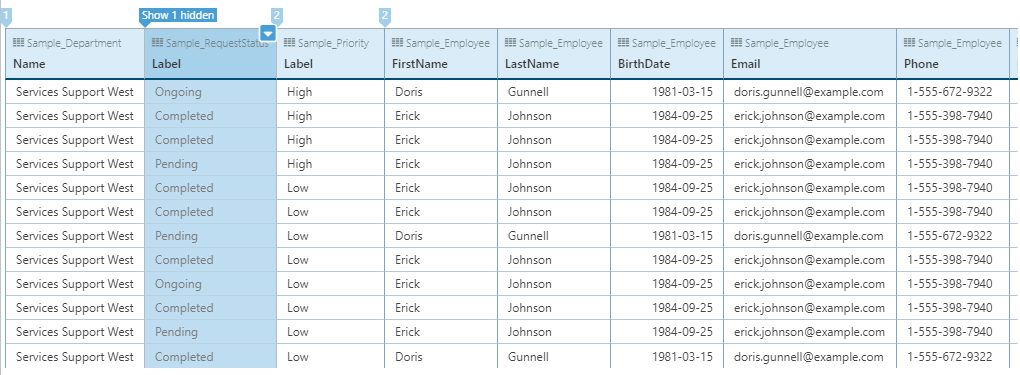
\includegraphics[height=2.0in]{hidden-attributes}
	\caption{Hidden attributes - primary and foreign keys are hidden by default.}
	\label{fig:hiddenAttributes}
\end{figure}

\begin{figure}[htbp]
	\centering
	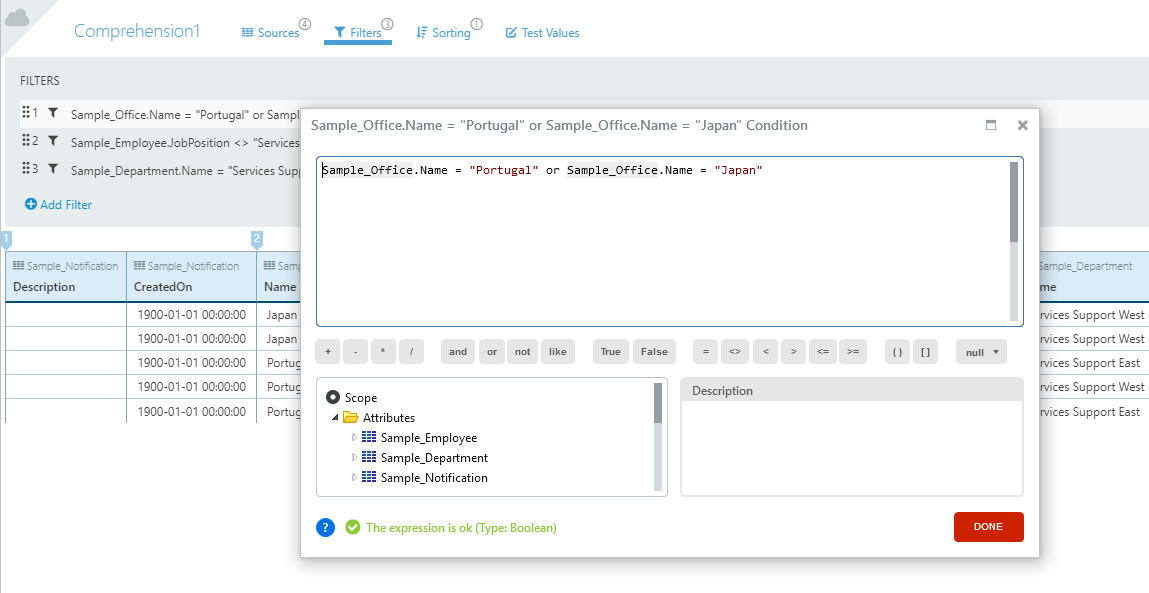
\includegraphics[height=2.5in]{aggregate-filter-modal}
	\caption{Filter edition modal - example of a filter edition after selection of the intended filter (the first one in that case).}
	\label{fig:aggregateFilterModal}
\end{figure}

\subsection{User Interviews}
\label{subsec:user_interviews}

After the analysis and study of the existing interface, there was a necessity to realize how are the usage of the visual query system for users. There was a demanding to comprehend what are the most impacting problems of the interface for users' tasks, what are the first users' reactions when asked about the utility of that interface, and if it could be applied, what are the reasons to use \gls{SQL} instead of OutSystems' visual query builder. Asking those general questions to users was the technique used to understand what is their in-depth and sincere opinion about the system utility and its most impacting problems.

Therefore, ten user interviews were performed to explore the tool's limits and understand their impact on user actions. The interviews started with some brief questions to perceive the background of the participant. After that, more directed questions were asked in order to understand the users' opinions about the advantages and disadvantages of the visual query tool. Besides, it was asked in which situations users prefer to use \gls{SQL} instead of the visual tool. The answer reveled to be important since it provided information about the main reasons to resort on \gls{SQL} alternative and also the main causes which led the user to stop using the visual query builder interface. Participants identified and demonstrated in-loco examples of limitations of the visual query system, highlighting causes and the impact of the problems. Also, users revealed other problems which have not been already identified.

Furthermore, the set of interviewed users, answered about which advanced functionalities would benefit further adoption and some usability problems previously identified. The purpose of these last questions was to ensure that the user answered truthfully about the aspects that most affect him negatively while using the visual query system. By letting him explain all the details about his vison, on further adjustments to the system, is possible to establish aspects of common groud between the conclusions of the primary analysis and the user reasoning about major limitations.

The results revealed that the most novice users, the users with less than six months of experience, consider Aggregates simple to use and stated that it covered their necessities, referring that it is more simple to learn than \gls{SQL}. The most experienced users, who use the OutSystems platform to develop applications, every day, for professional purposes, and have a technical technological background, reported that in the visual tool they cannot have a clear query understanding at a first glance. Moreover, they referred that they work with queries that contain several tables, attributes, and business rules. In those cases, they have considered that it was difficult to formulate queries using the visual querying interface. Besides, being required to switch between tabs in the interface to view the data sources, and the filters and sorts criteria, other issues were presented such as the lack of control on the query output\footnote{As referred on section \ref{subsubsec:current_progress}. When a user adds an entity to an Aggregate, all its attributes are added automatically and if the user hides them the output of the query does not change.}. When asked about the aggregation functions\footnote{Funtionality added when Simple Queries have been replaced by Aggregates (Section \ref{subsubsec:previous_work})}, they do not refer any problem with the approach interaction strategy adopted, but they have emphasized that it is very difficult to find the intended column that need, since there is no search or navigation engine. Other usability problems that decreases the users’ satisfaction, such as difficulty to search in all query or to copy and paste query components, were also pointed out.

In conclusion, the results of the problem definition phase indicated that the interface is simple to use but presents a considerable set of limitations in its components, mainly in the domain of professional purpose tasks. In that way, the suggestions to create an improved overview of the query, which would allow a faster comprehension of the query, as well as the implementation of interface accelerators to make the query editor powerful such as search engines and several access alternatives to the same functionality were the most stated aspects. Regardless of the suggestions, the user experience of the interface should be kept simple in order to continue to be easy to be learned and used by users without a technical technological background.

\subsection{Data Analysis}
\label{subsec:data_analysis}

Even though the analysis made and the first user interviews have indicated user experience problems of the interface as the factor that has been impacting the user acceptance of the visual query builder, a quantitative analysis was performed to perceive what are the operations most used by developers when they formulate queries textually. Thereby, the analysis was complemented with a metric study on queries executed on the Outsystems cloud, in order to find patterns that could justify users reasons to use \gls{SQL} instead of Aggregates. 

The queries analyzed, which have been extracted in July 2019 from customers’ projects, were built using Advanced Queries\footnote{The option of the OutSystems Platform, invoked in section \ref{subsubsec:previous_work}, that allows the query design in a textual way using a language based on \gls{SQL}.}. The data set used is composed of 214.400 statements. However, only 60.8\% were used in this study since only the queries are important for the results and not other SQL statements, such as inserts, updates, deletes, and transactions. Nevertheless, that set of 125.613 queries has duplicated results, so that these ones were removed resulting in a final data set of 67.828 queries. The operators and clauses were identified using a \gls{SQL} Parser developed in JavaScript \cite{jsSqlParser}. After obtaining the abstract syntax trees of the queries in a JSON file, that data was analyzed in a program to count the operators and the clauses that were present in the queries. 

Firstly, it was measured the percentage of \gls{SQL} queries that contained operations not supported by the visual tool. Table \ref{tab:aggregates_operations_not_supported_stats} summarizes the number and the percentage of those queries containing not supported operations. It is important to refer that the intersection of the subsets is not null, so there are queries that have two or more of the indicated operations. Nevertheless, it can be observed that most of the operations have no significant representation in the results. For example, the DISTINCT operation was the not supported operation with the highest percentage, included in 11.78\% of the queries analyzed.

%\begin{figure}[htbp]
%	\centering
%	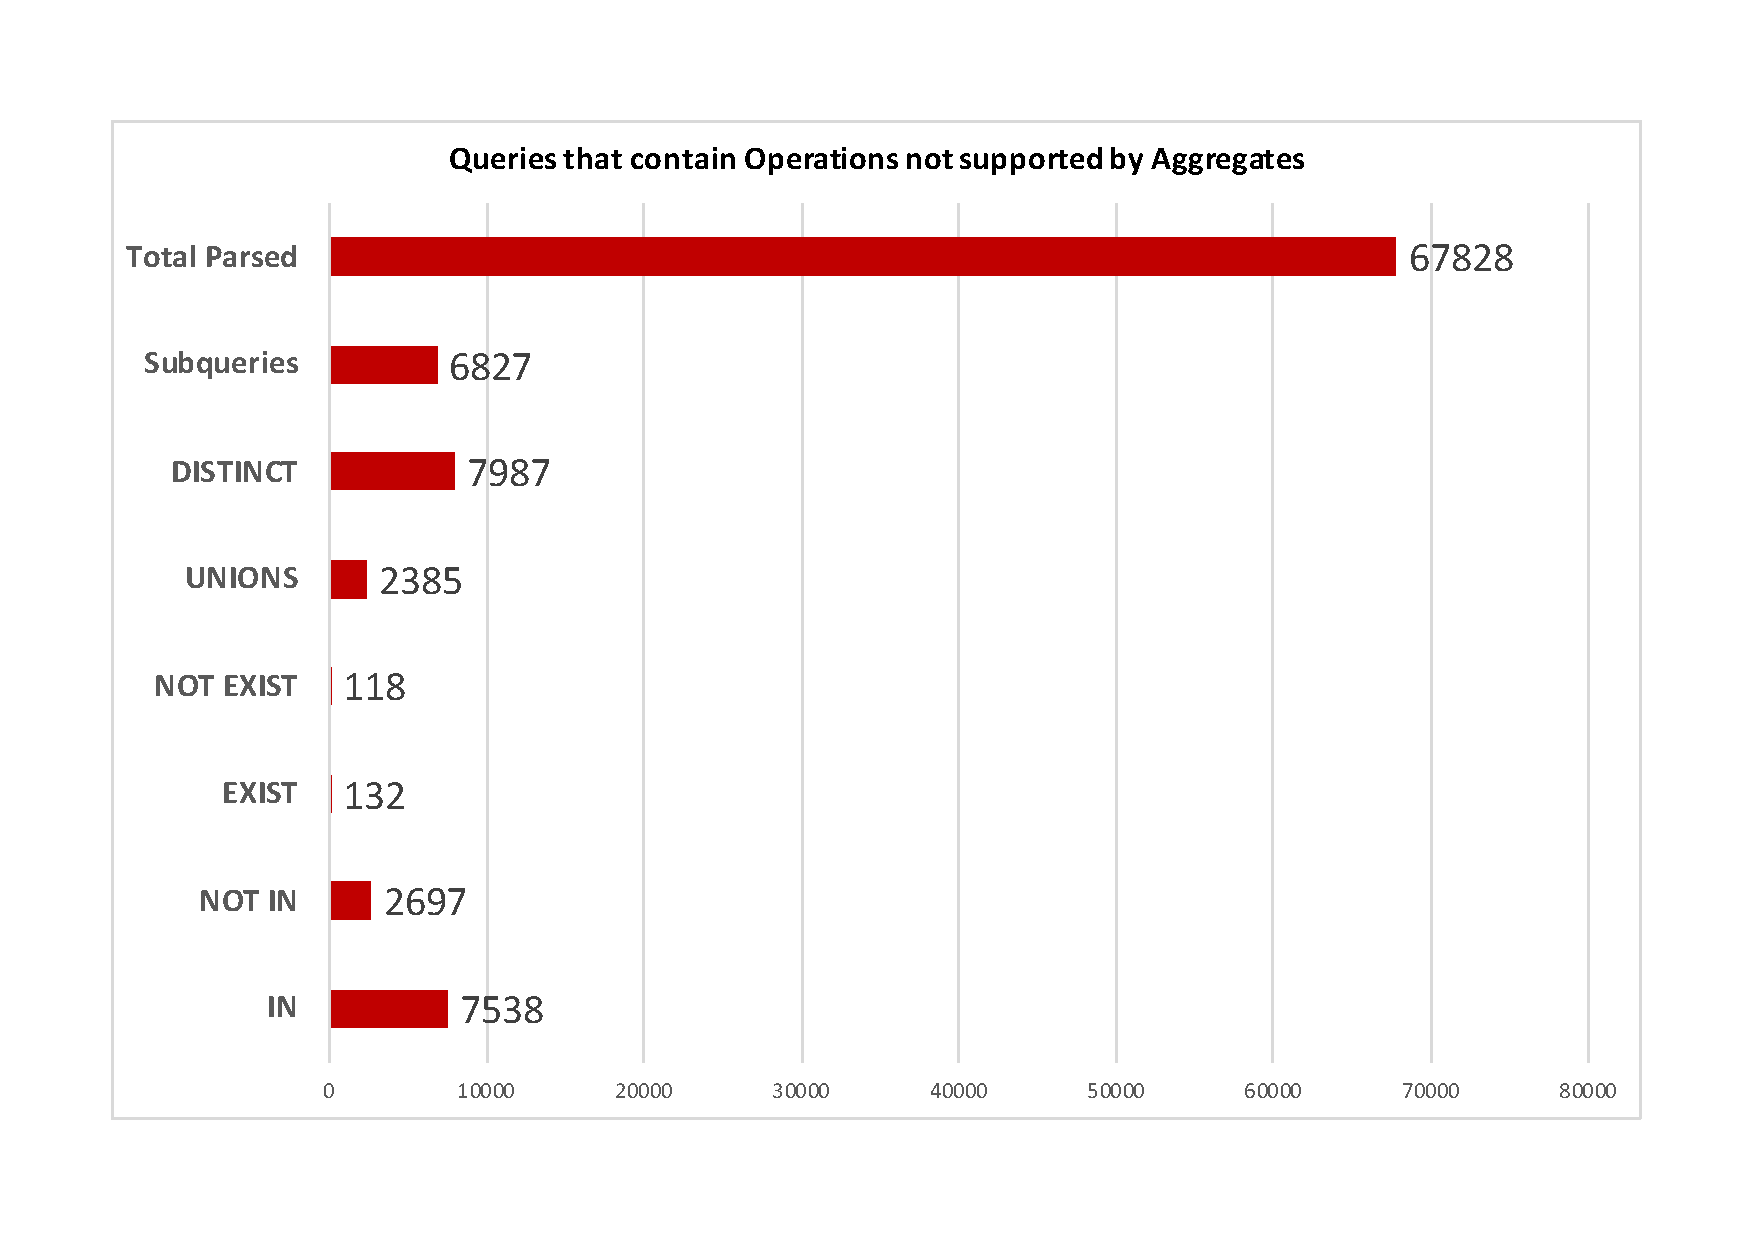
\includegraphics[height=3in]{ChartOperationsNotSupported}
%	\caption{Number of the queries that contain operations not supported by Aggregates}
%	\label{fig:aggregates_operations_not_supported_stats}
%\end{figure}

\begin{table}[tb]
	\caption{Queries that contain operations not supported by Aggregates}
	\label{tab:aggregates_operations_not_supported_stats}
\centering
\resizebox{\textwidth}{!}{
\begin{tabular}{c|c|c|c|c|c|c|c|c|}
    \cline{2-9}
    \rowcolor[HTML]{C0C0C0} 
    \cellcolor[HTML]{FFFFFF}                                 & IN      & NOT IN & EXIST  & NOT EXIST & UNIONS & DISTINCT & SUBQUERIES & Total \\ \hline
    \multicolumn{1}{|c|}{\cellcolor[HTML]{C0C0C0}Queries}    & 7538    & 2697   & 132    & 118       & 2385   & 7987     & 6827       & 67828 \\ \hline
    \multicolumn{1}{|c|}{\cellcolor[HTML]{C0C0C0}Percentage} & 11.11\% & 3.98\% & 0.19\% & 0.17\%    & 3.52\% & 11.78\%  & 10.07\%    & 100\% \\ \hline
    \end{tabular}
}
\end{table}

Secondly, it was measured how many queries were bluit using the textual language but could be designed using the visual query builder. Table \ref{tab:aggregates_supported_vs_not_supported_stats} shows the results obtained separating the queries performed in three categories:

\begin{itemize}
    \item Not Supported: Queries which include operations not supported by Aggregates, such as IN, NOT IN, EXIST, NOT EXIST, Unions, Distincts and Subqueries;
    \item Supported by Aggregates: Queries that could be designed totally using Aggregates. These are divided into two subcategories:
    \begin{itemize}
        \item Simpler: Queries which include only operations supported by aggregates excluding the indication of sorting criteria and the use of aggregation functions (e.g. GROUP BY or SUM, AVG, MIN, MAX, COUNT);
        \item More Complex: Queries that are supported by Aggregates excluding the above (simplers).
    \end{itemize}
\end{itemize}

User interviews suggested that aggregation functions and sorting criteria were not the main problems. Accordingly, the queries supported by Aggregates were divided into two groups in order to compare the quantitative analysis with the qualitative analysis extracted in interviews. This was considered an important element since these operations could be obtained using a different interaction technique where the user changes the query when he is interacting with the query result, as mentioned in section \ref{subsubsec:current_progress}. 

\begin{table}[tb]
	\caption{Queries that could be designed using Aggregates and the queries which the tool does not support}
	\label{tab:aggregates_supported_vs_not_supported_stats}
\centering
\resizebox{\textwidth}{!}{
\begin{tabular}{c|c|c|c|c|}
    \cline{2-5}
    \rowcolor[HTML]{C0C0C0} 
    \cellcolor[HTML]{FFFFFF}                                 & Not Supported & Supported (Simpler) & Supported (More Complex) & Total \\ \hline
    \multicolumn{1}{|c|}{\cellcolor[HTML]{C0C0C0}Queries}    & 28130         & 24026               & 15672                    & 67828 \\ \hline
    \multicolumn{1}{|c|}{\cellcolor[HTML]{C0C0C0}Percentage} & 41.5\%        & 35.4\%              & 23.1\%                   & 100\% \\ \hline
    \end{tabular}
    }
\end{table}

In the set of queries analyzed, around 58.5\% could be designed using Aggregates, is evident that the lack of support of some \gls{SQL} expressions might not be the main problem. Under the circumstances, the results were discussed together with the stakeholders. It was determined that the main problem was the usability of the system. 

In conclusion, the results of the quantitative analysis have confirmed the assumptions pointed out after the analysis and exploration of the interface and the first user interviews. All the studies made have concluded that the main priority of the project should be the usability improvement of the visual querying tool interface. Thereby, there are metrics that sustain the conclusions made in the problem definition phase.

\subsection{Community Ideas}
\label{subsec:community_ideas}

Since OutSystems has a wide worldwide Community of developers, the users can use the OutSystems Community Website \cite{outsystems_community} to express their problems or difficulties or even to communicate new ideas for the product. Thought that website, it was possible to extract information in order to align the final solution with the ideas and problems they shared. Accordingly, all 306 posts of category "Aggregates \& Queries" were analyzed in order to extract useful information for the design phase of this dissertation.

First of all, it has been taken into account for each post if the topic is related to the lack of some functionalities or related to some problems in the interface. That approach leads to perceive that the predominance of the posts were about usability problems of the interface, whereas there are a reduce quantity of posts about functionalities not supported.

Therefore, the users’ problems and suggestions regarding usability or enhancements of the interface were processed, transforming that information to a relevant input to the next design phases. All problems and suggestions identified were detailed in \nameref{app:taxonomy_of_problems_existing_interface}, followed with some examples of the problems and suggestions indicated in the OutSystems Community:

\begin{itemize}
    \item Search engines: users requested in multiple posts alternatives to search for an entity, attribute, or filter inside the query. Not only they refer that the readability in the interface is difficult primarily due to the non-existing color highlight in the text but also there is no possibility to search for the intended fields. They have also referred that this feature was extremely important for their work since they need to build queries with a large set of entities, attributes, and conditions;
    \item Filters Edition: it was pointed out in several posts suggestions to improve the interface in order to support filters comments with color highlighting, since they could be useful to explain the intention of the filter, or even the possibility to disable filters instead of deleting them.  
    \item Result Count: it was referred that there is no visible count of how many rows the query result has;
    \item Accelerators and Utilities: it has been suggested to add different accelerators in order to accelerate and streamline the query formulation process as well as different ways to present the query structure since, in the user's point of view, the query readability, provided with the existing interface, should be improved.
\end{itemize}

In summary, beyond the necessity of new advanced functionalities, the developers on the OutSystems Community have indicated different situations where the interface turns out not to be as powerful as it could be, since there is a lack of utilities or accelerators that could assist users keeping their task on track.

\subsection{Current Implementation Evaluation}
\label{sec:current_implementation_evaluation}

In order to analyze users' behavior while they are interacting with the visual query interface, testing scenarios were prepared to evaluate usability attributes of the interface.\footnote{This evaluation process is described in sections \ref{sec:testing_scenarios} and \ref{sec:evaluation_technique}.} The main purpose of this evaluation was the analysis of the current effectiveness, efficiency, and learnability of the system to compare them with the proposed solution. 

During the tests, users have mentioned other details of the interface that could be a useful input for the next design iterations. In that way, that feedback was also taken into account and registered as all the other issues identified. Thereby, \nameref{app:taxonomy_of_problems_existing_interface} includes also all problems identified during the user testing process of the existing visual query interface.


\section{Target Users}
\label{sec:target_users}

After obtaining a detailed and wide view of the existing problems, the following step was the exploration of how those problems can be solved. As the main goal is the development of an improved interface that gives to the users a solution to manage data queries efficiently, and effectively through intuitive interaction strategies, users are a crucial factor that must be taken into account throughout the entire solution development. Each user has his peculiarities, then the user experience of the solution should be adapted as much as possible to the target users of the query formulation system.

Considering that users will only use the visual query system if they use the OutSystems Platform, that low-code development context where the query system is inserted cannot be dissociated from the user analysis. Thereby, the user analysis process started by a study to categorize the profile of OutSystems Platform users according to the specificities of the data querying domain.

Since the low-code development paradigm has integrated more people who do not have the strict software engineer profile into software development tasks, the users of the OutSystems Platform do not have the same backgrounds, requirements, and expectations. If, on the one hand, there are OutSystems Developers that have Computer Science academic backgrounds or similar, and experience working with low-level programing language, on the other hand, there are business experts or specialized in other engineering fields that are also developing in OutSystems. In that way, the provided query building experience should be a hybrid approach that covers the traditional software developers demands without turning the development and the language intuitive for people that are not familiarized with classical development patterns, terminologies, or processes.

\subsection{Requirements and Expectations}
\label{subsec:requirements_and_expectations}

As the set of users that may use the visual query system is so broad and heterogeneous, it was necessary to analyze and register the aspects of the user profile which could branch out their needs and expectations in different directions. In this sense, the following three points of the users' background were considered the ones that could accurately cluster the users' expectations and demands, considering the usage context of the interface, which combines software development, low-code development, and relational databases querying domains:

\medskip

\textbf{Software Development Background:} The previous knowledge and experiences of users in the software development scope can lead significantly to their expectations while they are interacting with a graphical user interface. Being the object of study an interface that allows users to formulate queries, the factor mentioned becomes even more relevant. In software development, most users often associate database querying to languages that are considered a standard to perform those tasks, such as SQL. In that way, most users end up unconsciously relating the visual query building process to the languages they are familiar with. Therefore, if the visual query interface will be used by users that are familiar with technical languages, it is important to not forget to apply a language that could invoke similar principles and reasonings.

\medskip

\textbf{OutSystems Development Experience: } The user experience on low-code development, in particular using the OutSystems Platform, has also an impact on how the user will experience the visual data querying tool, even if the user does not build queries regularly through the Platform. As a complete solution for low-code development, the Service Studio has a consistent design across its sections. Consequently, a user familiarized with the Platform could have more facility to find options and understand interface language than a user that is using the Platform for the first time, since there are multiple design patterns and built-in behaviors across all the product.

Nevertheless, users who have considerable experience using the existing solution of OutSystems to build queries could be highly adapted to the existing design. Therefore, this fact should be taken into account throughout the solution design process in order to realize how modifications could impact regular users of the systems. Even knowing that frequent users could be skeptical of changes, it is necessary to properly assess whether the changes only require adaptation or if users could reject them. Therefore, it is important to improve the user experience of the existing interface without removing all its most representative features, in order to keep its singularity.

\medskip

\textbf{Data Tools Expertise: } Besides textual \glspl{DQL}, other tools allow users to manage and visualize data through graphical user interfaces. For instance, spreadsheet applications such as Microsoft Excel \cite{microsoftExcel} and Google Sheets \cite{googleSheets} presents an intuitive interface where users can manage, organize, and edit data. Using these interfaces, users do not need to know how relational databases work since data is presented in tables that could be manipulated directly under simple controls. For this reason, the language used in those systems is frequently less technical, in such a way that is important to consider that these users are expecting direct manipulation of data and simple language to query and manage data.


\subsection{User Groups}
\label{subsec:user_groups}

Being the relational database knowledge a crucial point to frame users' mental model of query formulation, it is important to split up the users who perceive relational databases to the other ones. On the other hand, low-code programming experience can affect how users interact with a visual programming system, thus it is important to study users with experience in low-code development through a different perspective. Considering the aspects mentioned, three user groups were created in order to cluster users that have similar profiles. Thereby, each user could integrate one of the following groups according to their characteristics:

\begin{table}[h]
    \caption{User Groups}
    \label{tab:user-groups}
    \begin{tabular}{|
    >{\columncolor[HTML]{C0C0C0}} m{3cm} |m{11cm}|}
    \hline
    \begin{tabular}[c]{@{}l@{}}Software \\ Developer\end{tabular}   & Software Developer or Engineer who has a solid previous knowledge of programming and databases. These users are familiarized with textual programming languages, such as C\#, SQL, and others. In that way, they cannot abstract their previous knowledge in such a way that communication with these users should be more technical and specific. Finally, this user group is not an expert in low-code development. However, as they have solid programming, logic, and database knowledge, they could develop some applications using low-code if necessary. \\ \hline
    \begin{tabular}[c]{@{}l@{}}OutSystems \\ Developer\end{tabular} & Independently of their background, these users are experienced in OutSystems. That way, they are proficient and faster in low-code development, regardless of their experience in other traditional software development paradigms. This is your principal characteristic that should be taken into account. \\ \hline
    \begin{tabular}[c]{@{}l@{}}Citizen \\ Developer\end{tabular}    & Users who do not have an extensive programming or software development background. Even though they are not software developers, they could develop some simple apps using low-code due to its simplicity. As some of these users may not know how relational databases work, they may use other applications, such as Microsoft Excel, Google Sheets, Salesforce, and others to manage data. \\ \hline
    \end{tabular}
\end{table}

%Furthermore, users tend to adapt their expectations in consonance with design patterns they found in software which they usually use. That is important because the tools often used to complete programming tasks, such as \glspl{IDE} or powerful Text Editors, have a set of features to facilitate users to reach the intended tasks. For instance, search engines, syntax highlighting, and keyboard accelerators not only assist users to keep their tasks on track, but also reduce the time needed to complete each task. Thereby, these users will feel disappointed if they need to use a query builder interface that does not have these productive features to turn the query formulation process more straightforward and efficient.


%Regarding database querying, these users have a tendency to focus the query formulation process on data structure more than on the query output. 

%Key Points:
%------------------------------------
%--Software Development Background
%-O background do utilizador no âmbito das tarefas ligadas ao desenvolvimento de software, tanto de um ponto de vista de aprendizagem como de experiência prática podem influenciar bastante as suas espectativas na interação com a interface gráfica em estudo. Não só por muitas vezes estes utilizadores associarem diretamente o domínio de data querying a linguagens que são utilizadas há largos anos, como o SQL, mas também pelo tipo de software que usam no contexto do desenvolvimento de software que acaba por encaminhas as espectativas do utilizador num sentido. Tal como referido, o SQL tem sido a linguagem de querying mais utilizada ao longo dos últimos anos, tendo até sido considerada como a linguagem de querying standard. Portanto, o que é relevante destacar é que o facto dos utilizadores conhecerem e estarem habituados a utilizar esta interface poder impactar a interação com a interface visual de querying, uma vez que será considerada muitas vezes como o ponto de referência no ato de construção de consultas a bases de dados. 
%-Para além disso, o software que os profissionais de desenvolvimento de software utilizam no seu dia a dia (text editors or IDEs), acabam por apresentar características que podem modificar a espectativa do utilizador na forma como espera que o sistema responda. Por exemplo quando os utilizadores utilizam um software de edição de texto que possui aceleradores de procura, color hightlighting e shortcuts o processo de construção de consulta a bases de dados acaba por ser mais rápido, aumentando o nível de satisfação do utilizador. Deste modo, é necessário considerar que os utilizadores que tem conhecimento de SQL estão habituados a ter este tipo de mecanismos que auxiliam a construção de queries.
%-
%-
%-Não só a consulta de dados está muitas vezes aliada ao procesos de desenvolvimento de software, mas também
%-Vão sempre ter como base outras tecnologias para realizar consultas a bases de dados (SQL)
%-Estão habituados a poder manipular todos os aspetos da query de forma fácil e rápida (Experiência do IDE)
%-
%--OutSystems Development Experience
%-------------------------------------
%-A experiência de desenvolvimento de software através da plataforma OutSystems acaba por influenciar a forma como o utilizador se irá sentir ao utilizar a solução visual de data querying. Mesmo que o utilizador não tenha muita experiência em usar os Aggregates, o Service Studio, como IDE possuí consistência nos mecanismos de interação usado na comunicação com o utilizador. Assim sendo, um utilizador habituado a utilizar o Service Studio não irá talvez identificar ou questionar certos comportamentos do sistema por já estar habituado à presença dos mesmos. Para além disso, o facto do utilizador já ter ou não usado os Aggregates é um dado importante para a análise do utilizador uma vez que estes utilizadores poderão usar a nova interface mantendo um pensamento de comparação com a anterior.
%
%-Habituados aos padrões de experiência existentes no Service Studio
%-Habituados à experiência antiga dos aggregates
%-
%--Data Tools Expertise
%-Para além das linguagens de querying textuais, existem muitas ferramentas com interface gráfica que permitem que os utilizadores giram e visualizem os seus dados. A natureza e o propósito destes softwares podem ser bastante distintos, pois um podem-se aplicar mais à gestão e organização dos dados (Access, Excel or Google Spreasheets) e outros à visualização dos mesmos (Microsoft Power BI ou Tableau). No entanto, este tipo de ferramentas foca-se muito na natureza dos dados e não tanto na sua estrutura de um ponto vista de modelação de dados, ao contrário do SQL. Assim sendo, é importante perceber a forma como o utilizador orienta o seu raciocínio relativamente a gestão de dados, e para isso a sua experiência de utilização de data tools é importante para a análise do perfil do utilizador.
%
%-Foco nos dados em vez de na estrutura (Data visualization tools e excel) 
%-
%-

%-De acordo com os pontos referidos, os utilizadores foram divididos em três grupos de modo a poder-se analisar o impacto das alterações efetuadas nos utilizadores quer têm diferentes perspetivas de utilização do sistema.
%-
%-Assim sendo, cada utilizador que testa o sistema deve ser integrado num dos seguintes grupos, de acordo com as suas características.
%-


% \clearpage


% \section{Proposed Implementation}
% \label{sec:proposed_implementation}
% According to the analysis made and the results concluded, the implementation covers an iterative design process aiming at improving the usability of Aggregates, the component of the OutSystems Platform to visually build queries. The prioritized improvements of the \gls{VQL} expressiveness (IN / NOT IN and DISTINCT) will be included in the project, if possible, depending on the development progress of the usability issues. If in the next stages of development it is found that it is possible to address these expressiveness problems without impairing the development related to improving usability, these will be designed and developed, otherwise, the focus will be only the usability improvement. %TODO: Falta explicar melhor em que consiste melhorar a usabilidade, resumindo quais sao os problemas

% As mentioned above in Section \ref{subsubsec:current_progress}, the actual visual tool include in the interface sections to design queries visually and to view their results. Therefore, the aim is to design and evaluate how these two parts of the interface can be changed to improve the usability of the system. In a nutshell, there are two aspects that are needed to be taken into account, in order to guide the design process: the simplicity, efficiency and effectiveness to construct queries independently of how many tables or conditions, and the readability of the global query to perceive what data of the database the query will be gathering.

% %Never forgetting these guidelines, the query parts specified in Table X will guide the design process, studying and evaluating solutions to improve the specification method, without harming the query overview readability and the interaction strategies to specify the other parts of the query. 

% The design and development process shall be divided into an initial preparation and analysis phase and the iterative design process phase:

% \begin{itemize}
%     \item \textbf{Preparation and analysis phase}: before the development of the prototypes, the users and the tasks of the should be analyzed. Also, it should be started sketching as a means to bring up ideas that could represent starting points to tackle the existing problems. Therefore, this preparation process before the development of the prototypes will include the following tasks:
%     \begin{itemize}
%         \item \textbf{Data Extraction}: although there are results obtained in the interviews and in the quantitative analysis process, detailed in \ref{sec:requirements_analysis}, additional data about the queries design using aggregates also will be extracted. It could be important to the process to understand the user's usage of the existing visual tool since the results obtained are only about the queries built using the textual language;
%         \item \textbf{User and Task Analysis}: users and their tasks will be characterized and classified regarding the concepts presented in section \ref{subsubsec:user_and_task_analysis} This description and classification will be used not only as a reference point throughout the design process but also to define the most important trade-offs on usability attributes;
%         \item \textbf{Sketching}: the phase where the first sketches of possible solutions will be designed. The most important is the initial exploration of several possibilities to tackle the problems through a low-level and fast approach. As referred in section \ref{subsubsec:sketching_and_prototyping} it is useful to discover new ideas, keeping register the first approaches to tackle the problems. At the later phases, the sketches could be useful to remember the starting point of the design process;
%     \end{itemize}
%     \item \textbf{Iterative design}: this process starts with low-level prototypes and in each iteration, these are evaluated to create higher fidelity prototypes in the next iteration. However, as referred in section \ref{subsubsec:sketching_and_prototyping}, there are different strategies to reuse or not the prototypes over iterations. In this project, an evolutionary strategy where the prototypes developed are used as the basis for the next design iteration will be adopted. Moreover, the design process will include three iterations:
%     \begin{itemize}
%         \item \textbf{Paper Prototype (1st iteration)}: regarding the information obtained in user and task analysis, and the main ideas raised on the sketching stage, a first functional paper prototype will be built. The evaluation of the entire concept of the first interaction strategies is the main concern of this phase. Cognitive Walkthrough and Observational Methods of user testing will be the evaluation techniques used on this phase;
%         \item \textbf{Low-fidelity Prototype (2nd iteration)}: using the results of the previous iteration, the idea is to develop a low-fidelity computer prototype on technologies, such as Balsamiq \cite{balsamiq} or Mockingbird \cite{mockingbird}, which although do not create native applications, allow the employment of visual components and animations more similar with the intended in the final solution. So, more aspects can be tested regarding a higher complexity and fidelity of the interface. At this stage, Heuristic Evaluation will be used by experts and more user tests will be performed. However, it is likely that not only Observational Methods are performed. Experimental Methods could be necessary to test specific hypotheses or discuss what is the better option between a set of possible implementations. Moreover, Query Methods, like questionnaires, could be valuable as well, to understand the user’s satisfaction;
%         \item \textbf{Final Prototype (3rd iteration)}: computer prototype integrated in the OutSystems Platform. The development focuses on the presentation layer of the application due to improving the Aggregates interface and \gls{UX}, using the new results obtained. The front-end of the application is developed in React \cite{react}, using the TypeScript \cite{typescript} language. Accordingly, these are the technologies that will be used in the development of the final prototype. Being the last prototype and consequently the final result of this project, it will be evaluated also by users and experts to summarize the final results of all the design and development process;
%     \end{itemize}

% \end{itemize}

% \section{Work Plan}
% \label{sec:work_plan}
% According to the proposed implementation approach, Figure \ref{fig:work_plan} represents a work plan until the final of the thesis, scheduling each one of the tasks explained in the previous section throughout the remaining weeks. The tasks are assigned to its respective major phases, and the focus on the writing of the document is primarily at the end of each phase or iteration to summarize all the contents addressed during these periods, although the report can be updated every time it reveals useful.

% \begin{figure}[hb]
% 	\centering
% 	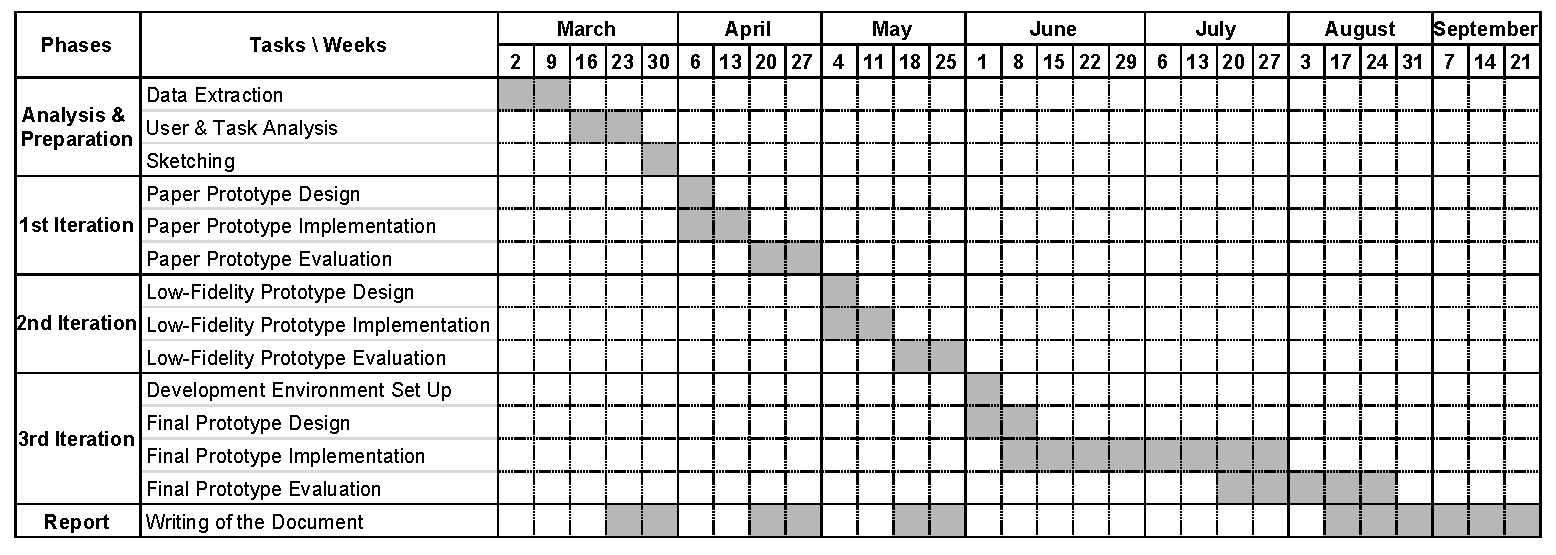
\includegraphics[width=1.0\textwidth]{workPlan}
% 	\caption{Task Scheduling throughout the weeks until the final of the project.}
% 	\label{fig:work_plan}
% \end{figure}



